\section{Procedure}

\begin{tcolorbox}[
  colback=blue!5,
  colframe=blue!40,
  breakable,
  title=Box 2 | Quickstart: single-display example workflow,
  fonttitle=\bfseries
]

The following workflow reproduces the complete DELT-Hit analysis for the single-display example dataset provided in the supporting material (see Section~3.3 Data). It is intended as a self-contained reference for users who want to run through the entire pipeline on the provided example before adapting it to their own data. This workflow produces the outputs presented in the Anticipated Results section. DELT-Hit needs to be installed as described in Box~1.

\setupitem{Download the repository and enter the example directory}

\begin{lstlisting}
git clone https://github.com/DELTechnology/delt-hit.git
cd delt-hit/supporting_material/experiments/example-single-display
\end{lstlisting}

\setupitem{Download the example data}

\begin{lstlisting}
cd supporting_material/experiments/example-single-display
bash download.sh
\end{lstlisting}

\setupitem{Initialize the configuration}

\begin{lstlisting}
delt-hit init --excel_path=example-single-display.xlsx
CONFIG_PATH=campaign/config.yaml
ANALYSIS_CONFIG_PATH=analysis.yaml
ANALYSIS_OUTPUT_ROOT=campaign/analysis
\end{lstlisting}

\setupitem{Demultiplexing}

\begin{lstlisting}
delt-hit demultiplex prepare --config_path="$CONFIG_PATH"
bash campaign/demultiplex/cutadapt_input_files/demultiplex.sh
delt-hit demultiplex report --config_path="$CONFIG_PATH"
delt-hit demultiplex qc --config_path="$CONFIG_PATH"
delt-hit demultiplex process --config_path="$CONFIG_PATH"
delt-hit demultiplex process --config_path="$CONFIG_PATH" --as_files=True
\end{lstlisting}

\setupitem{Library enumeration and visualization}

\begin{lstlisting}
delt-hit visualize enumerate --config_path="$CONFIG_PATH"
delt-hit library enumerate \
  --config_path="$CONFIG_PATH" \
  --counts_path=campaign/selections/AG24_4/counts.txt \
  --top_n=1000 \
  --library_name=AG24_4_top_hits
delt-hit visualize library --config_path="$CONFIG_PATH" \
  --library_name=AG24_4_top_hits
delt-hit library properties --config_path="$CONFIG_PATH" \
  --library_name=AG24_4_top_hits
delt-hit dashboard \
  --config_path="$CONFIG_PATH" \
  --counts_path=campaign/selections/AG24_4/counts.txt
\end{lstlisting}

\setupitem{Enrichment analysis}

\begin{lstlisting}
delt-hit analyse enrichment \
  --analysis_config="$ANALYSIS_CONFIG_PATH" \
  --name=condition_vs_control --method=counts \
  --save_dir="$ANALYSIS_OUTPUT_ROOT"
Rscript --vanilla "$ANALYSIS_OUTPUT_ROOT/counts/condition_vs_control/enrichment_counts.R"

delt-hit analyse enrichment \
  --analysis_config="$ANALYSIS_CONFIG_PATH" \
  --name=condition_vs_control --method=edgeR \
  --save_dir="$ANALYSIS_OUTPUT_ROOT"
Rscript --vanilla "$ANALYSIS_OUTPUT_ROOT/edgeR/condition_vs_control/enrichment_edgeR.R"

for selection in AG24_13 AG24_14 AG24_15; do
  delt-hit analyse enrichment \
    --config_path="$CONFIG_PATH" \
    --counts=campaign/selections/$selection/counts.txt \
    --method=z_score --name=$selection \
    --save_dir="$ANALYSIS_OUTPUT_ROOT"
  Rscript --vanilla "$ANALYSIS_OUTPUT_ROOT/z_score/$selection/enrichment_z_score.R"
done
\end{lstlisting}

\setupitem{Full library enumeration and molecular representations}

\begin{lstlisting}
delt-hit library enumerate --config_path="$CONFIG_PATH"
delt-hit library properties --config_path="$CONFIG_PATH"
delt-hit library represent --method=morgan --config_path="$CONFIG_PATH"
delt-hit library represent --method=bert --config_path="$CONFIG_PATH"
\end{lstlisting}

\end{tcolorbox}

\subsection{Phase 1 | Project initialization and configuration}

\textbf{TIMING:} 15--60 min

<CRITICAL>: In this phase, a YAML configuration file is created from an Excel workbook that contains the DEL and experimental design information. The following steps describe the required sheets and their format. We recommend starting from the provided example workbook provided on Github (under \texttt{templates}) and adjusting it to the new library.


\protocolstep{1}{Create the experiment sheet}

Table~\ref{tab:table3} shows the complete layout of the \texttt{experiment} sheet. Required fields of the \texttt{experiment} sheet are as follows: 

\begin{itemize}
  \item \texttt{name}: Experiment name
  \item \texttt{fastq\_path}: File path
  \item \texttt{save\_dir}: Folder to which DELT-Hit outputs are written to, created under \texttt{save\_dir} and named \texttt{\textless name\textgreater}
  \item \texttt{num\_cores}: Defines the number of CPU cores used for the demultiplexing step
\end{itemize}

\begin{table}[htbp]
\centering
\caption{Experiment configuration parameters}
\label{tab:table3}
\begin{tabular}{ll}
\toprule
variable & value \\
\midrule
name & campaign \\
fastq\_path & campaign.fastq.gz \\
save\_dir & ./ \\
num\_cores & 11 \\
\bottomrule
\end{tabular}
\end{table}


<CRITICAL> Use absolute paths, or paths relative to the working directory, for \texttt{fastq\_path} and \texttt{save\_dir}. Here, \texttt{./} refers to the current working directory from which the command is run.


\protocolstep{2}{Create the selection sheet}

Define the experimental design within this sheet, like selection conditions, multiplexing barcodes and replicate grouping. Table~\ref{tab:table4} shows an example layout. Required columns for demultiplexing:

\begin{itemize}
  \item \texttt{name}: Unique identifier for each selection
  \item \texttt{S0}, \texttt{S1}: Multiplexing barcodes for selection identification
\end{itemize}
Optional columns:

\begin{itemize}
  \item \texttt{group}: Statistical grouping when needed for downstream analyses (for example, "condition" or "control")
  \item \texttt{operator}: Person who performed the selection
  \item \texttt{date}: Date of selection experiment
  \item other columns can be added at the user's discretion
\end{itemize}

\begin{table}[htbp]
\centering
\caption{Selection experimental design}
\label{tab:table4}
\begin{tabular}{lllllll}
\toprule
name & operator & date & group & target & S0 & S1 \\
\midrule
AG24\_4 & A. Smith & 26-Sep-24 & no\_condition &  & ACACAC & TCGATA \\
AG24\_5 & A. Smith & 26-Sep-24 & no\_condition &  & ACAGCA & TCGATA \\
AG24\_6 & A. Smith & 26-Sep-24 & no\_condition &  & ACATGT & TCGATA \\
AG24\_13 & A. Smith & 26-Sep-24 & condition & A & ACGACG & TCGATA \\
AG24\_14 & A. Smith & 26-Sep-24 & condition & A & ACGCGA & TCGATA \\
AG24\_15 & A. Smith & 26-Sep-24 & condition & A & ACTAGC & TCGATA \\
\bottomrule
\end{tabular}
\end{table}

\protocolstep{3}{Create the structure sheet}

Define the DNA construct architecture and error tolerances for demultiplexing. Each DNA region is identified by a unique name across three types of DNA regions:

\begin{itemize}
  \item \texttt{selection}: Region used for selection primers defined in the \texttt{selection} sheet. These regions should be named \texttt{S0} and \texttt{S1}.
  \item \texttt{constant}: Constant regions shared across DNA constructs. These regions should be named sequentially \texttt{C0}, \texttt{C1}, ..., \texttt{CN}.
  \item \texttt{building\_block}: Region identifying a chemical building block. These regions should be named sequentially \texttt{B0}, \texttt{B1}, ..., \texttt{BN}.
\end{itemize}

Table~\ref{tab:table5} summarizes the expected layout. The following columns and parameters are to be defined: 

\begin{itemize}
  \item \texttt{name}: Unique identifier for each DNA region
  \item \texttt{type}: Region type (\texttt{selection}, \texttt{constant}, or \texttt{building\_block})
  \item \texttt{max\_error\_rate}: Maximum allowed error rate for adapter trimming (0 = perfect match, 0.1 = 10\% errors), can be configurated separately for each region
  \item \texttt{indels}: Whether to allow insertions/deletions (\texttt{TRUE}/\texttt{FALSE})
  \item \texttt{reverse}: Whether to reverse the codon before matching (\texttt{TRUE}/\texttt{FALSE}; mostly relevant for dual-display libraries)
  \item \texttt{complement}: Whether to complement the codon before matching (\texttt{TRUE}/\texttt{FALSE}; mostly relevant for dual-display libraries)
\end{itemize}

\begin{table}[htbp]
\centering
\caption{DNA sequence structure definition}
\label{tab:table5}
\begin{tabular}{llllll}
\toprule
name & type & max\_error\_rate & indels & reverse & complement \\
\midrule
S0 & selection & 0 & FALSE & FALSE & FALSE \\
C0 & constant & 1.01 & FALSE & FALSE & FALSE \\
B0 & building\_block & 0 & FALSE & FALSE & FALSE \\
C1 & constant & 1.01 & FALSE & FALSE & FALSE \\
B1 & building\_block & 0 & FALSE & FALSE & FALSE \\
C2 & constant & 1.01 & FALSE & FALSE & FALSE \\
S1 & selection & 0 & FALSE & FALSE & FALSE \\
\bottomrule
\end{tabular}
\end{table}


<CRITICAL> To balance assignment accuracy and read recovery, we recommend using exact matching for barcodes while allowing for 1--2 errors in constant regions. For advanced error configuration we refer to the Cutadapt \cite{martin_cutadaptremovesadapter_2011} documentation.


\protocolstep{4}{Create the constant sheet}

Insert the DNA sequences for all constant regions defined in the \texttt{structure} sheet, as illustrated in Table~\ref{tab:table6}.

\begin{table}[htbp]
\centering
\caption{Constant DNA region sequences}
\label{tab:table6}
\begin{tabular}{ll}
\toprule
name & codon \\
\midrule
C0 & GGAGCTTCTGAATTCTGTGTGCTG \\
C1 & CGAGCGTCAGGCAGCCTGTGTGCTG \\
C2 & CGAGTCCCATGGCGC \\
\bottomrule
\end{tabular}
\end{table}

<CRITICAL> The \texttt{name} column must match the constant-region names defined in the \texttt{structure} sheet.

\protocolstep{5}{Create building block sheets}

For each barcode region defined in the structure sheet, create a separate sheet named sequentially as \texttt{B0}, \texttt{B1}, ..., \texttt{BN} and list the DNA codons used at that position. To enable library enumeration and property calculation, also define the chemical structures of the building blocks and the reactions used during library synthesis. Table~\ref{tab:table7} gives a representative example.

Required columns for demultiplexing:

\begin{itemize}
  \item \texttt{codon}: DNA barcode sequence identifying this building block
\end{itemize}
Optional for demultiplexing, required for enumeration:

\begin{itemize}
  \item \texttt{smiles}: Chemical structure in SMILES notation
  \item \texttt{reaction}: Name of the reaction using this building block
  \item \texttt{educt}: Name of the compound this building block reacts with if any
  \item \texttt{product}: Name of the product formed
\end{itemize}

\begin{table}[htbp]
\centering
\caption{Building block definition sheet (example for B0)}
\label{tab:table7}
\begin{tabular}{lllll}
\toprule
codon & smiles & educt & reaction & product \\
\midrule
ATCTAT & NCC1=CC=CS1 & scaffold\_1 & ABF1 & product\_1 \\
AGAATA & COC1=CC=C(OC)C(CN)=C1 & scaffold\_1 & ABF1 & product\_1 \\
TCATTA & NCCCSCC1=CC=C(F)C=C1 & scaffold\_1 & ABF1 & product\_1 \\
TTGACT & NCC1(CC1)C1=CC=CC=C1 & scaffold\_1 & ABF1 & product\_1 \\
\bottomrule
\end{tabular}
\end{table}

\begin{tcolorbox}[
  colback=gray!10,
  colframe=gray!50,
  title=Box 3 | SMILES and SMIRKS,
  fonttitle=\bfseries
]
SMILES (Simplified Molecular Input Line Entry System) is a text notation for representing the structure of an individual molecule. In DELT-Hit, each building block is provided as a SMILES string in the corresponding \texttt{B0}, \texttt{B1}, ..., \texttt{BN} sheet so that the software can reconstruct products and calculate molecular properties. For example, the SMILES string \texttt{NCC1=CC=CS1} describes a small molecule that contains an aminoethyl side chain attached to a five-membered aromatic ring with sulfur. At a high level, a SMILES string tells the software which atoms are present and how they are connected in the molecule.

\begin{center}

\includegraphics[width=0.35\textwidth]{figures/structure.png}
\end{center}

SMIRKS is a reaction notation derived from SMARTS that describes how one or more reactants are transformed into a product. In DELT-Hit, SMIRKS definitions are used to encode the chemistry of each library-synthesis step so that building blocks can be combined in silico during library enumeration. For example, the \texttt{ABF1} reaction in Table~\ref{tab:table8} encodes an amide bond formation between a carboxylic acid and an amine:

\begin{lstlisting}
[CX3:1](=[O:2])[OX2;H1].[N;$([N;H1,H2]),$([N;H3]);!$([N;H1,H2][S]);
  !$([NX3][CX3](=[OX1])[#6]);!$([NX3][CX3](=[OX1])[OX2]):4]
  >>[CX3:1](=[O:2])[N:4]
\end{lstlisting}
At a high level, the left side specifies the reacting functional groups, and the right side specifies how they are connected in the product. In practice, SMILES \cite{ref33} describes molecules, whereas SMIRKS \cite{ref34} describes transformations between molecules.
\end{tcolorbox}

\protocolstep{6}{Create the reactions sheet}

<CRITICAL> Before attempting to enumerate an entire library, we recommend a validation of all reaction notations with a representative subset of building blocks. SMIRKS should be specified so that each transformation yields a single product.

In the \texttt{reactions} sheet, define all chemical reactions used during library synthesis with SMIRKS notation\cite{ref34}. For reaction types used at multiple stages of library synthesis, define each instance as a separate reaction to simplify inspection of the produced reaction graph. Table~\ref{tab:table8} illustrates this with two amide-bond-forming reactions (\texttt{ABF1} and \texttt{ABF2}). 

\begin{table}[htbp]
\centering
\caption{Reaction SMIRKS templates}
\label{tab:table8}
\begin{tabular}{p{1.5cm}p{13.0cm}}
\toprule
Name & SMIRKS \\
\midrule
ABF1 & {\footnotesize\ttfamily\seqsplit{[CX3:1](=[O:2])[OX2;H1].[N;\$([N;H1,H2]),\$([N;H3]);!\$([N;H1,H2][S]);!\$([NX3][CX3](=[OX1])[\#6]);!\$([NX3][CX3](=[OX1])[OX2]):4]>>[CX3:1](=[O:2])[N:4]}} \\
ABF2 & {\footnotesize\ttfamily\seqsplit{[CX3:1](=[O:2])[OX2;H1].[N;\$([N;H1,H2]),\$([N;H3]);!\$([N;H1,H2][S]);!\$([NX3][CX3](=[OX1])[\#6]);!\$([NX3][CX3](=[OX1])[OX2]):4]>>[CX3:1](=[O:2])[N:4]}} \\
SR & {\footnotesize\ttfamily\seqsplit{[\#6:1][\$([NX2-][NX2+]\#[NX1]),\$([NX2]=[NX2+]=[NX1-])]>>[\#6:1][N;H2]}} \\
CuAAC & {\footnotesize\ttfamily\seqsplit{[CX2:1]\#[CX2;H1:2].[N:3]=[N+:4]=[N-:5]>>[C:1]1=[C:2][N-0:3][N-0:4]=[N-0:5]1}} \\
\bottomrule
\end{tabular}
\end{table}


<CRITICAL> The \texttt{name} column must match the reaction names used in the building block sheets \texttt{B0}, \texttt{B1}, ..., \texttt{BN}.

\protocolstep{7}{Create the compounds sheet}

Define any additional chemical compounds (scaffolds, reactants) used for library enumeration, as shown in Table~\ref{tab:table9}.

\begin{table}[htbp]
\centering
\caption{Compound definitions}
\label{tab:table9}
\begin{tabular}{ll}
\toprule
name & smiles \\
\midrule
scaffold\_1 & O=C(N)CCC(N=[N+]=[N-])C(O)=O \\
\bottomrule
\end{tabular}
\end{table}

\protocolstep{8}{Create the additional reaction steps}

<CRITICAL> If library synthesis includes additional steps, such as precursor conversion or deprotection before a reaction, define them in the \texttt{reaction\_graph} sheet.


Define each additional reaction as a separate row with up to two educts, a reaction name, and the resulting product. Use the compound and reaction names defined in the corresponding sheets. Table~\ref{tab:table10} shows the general format.

\begin{table}[htbp]
\centering
\caption{Additional reaction step definitions}
\label{tab:table10}
\begin{tabular}{llll}
\toprule
educt\_1 & educt\_2 & reaction & product \\
\midrule
product\_1 &  & SR & product\_1B \\
\bottomrule
\end{tabular}
\end{table}

<PAUSE POINT> The generated Excel workbook can be adapted to other experiments by modifying the experiment and selection sheets, provided the underlying library remains unchanged.

\protocolstep{9}{Generate the configuration file}
Once your Excel file is complete with all required sheets, activate the DELT-Hit environment and generate the YAML configuration file:


\begin{lstlisting}
conda activate delt-hit
delt-hit init --excel_path=<PATH_TO_EXCEL>
\end{lstlisting}

Review the generated YAML file at \texttt{\textless save\_dir\textgreater/\textless name\textgreater/config.yaml}, as defined in the \texttt{experiment} sheet to verify that all information was parsed correctly. This file is used in all downstream steps.

<CRITICAL>: Throughout the following steps, angle-bracket tokens such as \texttt{\textless name\textgreater}, \texttt{\textless save\_dir\textgreater}, \texttt{\textless selection\_name\textgreater}, and \texttt{\textless library\_name\textgreater} are placeholders to be replaced with values from the Excel workbook or analysis YAML. \texttt{\textless name\textgreater} and \texttt{\textless save\_dir\textgreater} refer to the fields in Table~\ref{tab:table3}; \texttt{\textless experiment\_name\textgreater} and \texttt{\textless selection\_name\textgreater} refer to the \texttt{name} fields in the analysis YAML defined in Step~17.

\textbf{$\blacklozenge$ Troubleshooting}

\subsection{Phase 2 | Sequence processing and demultiplexing}

\textbf{TIMING:} 1--2 h

<CRITICAL>: This phase processes raw sequencing reads to identify and count each library member in your selection experiments. 

\protocolstep{11}{Prepare and execute sequence demultiplexing}
Generate the demultiplexing scripts with its input files by running

\begin{lstlisting}
CONFIG_PATH=<save_dir>/<name>/config.yaml
delt-hit demultiplex prepare --config_path=$CONFIG_PATH
\end{lstlisting}

Execute demultiplexing script that runs Cutadapt against the FASTQ file, maps reads to selection and codon identifiers, and outputs all mapped sequences to \texttt{reads\_with\_adapters.gz}.

\begin{lstlisting}
<save_dir>/<name>/demultiplex/cutadapt_input_files/demultiplex.sh
\end{lstlisting}

\textbf{$\blacklozenge$ Troubleshooting}

\protocolstep{12}{Inspect demultiplexing quality}
Generate the demultiplexing report and QC figures. The report (Figure~\ref{fig:figure4}) relates read retention across demultiplexing stages. The generated QC plots (Figure~\ref{fig:figure5}) show barcode-level plots for each indexed region.

\begin{lstlisting}
# Generate quality control report
delt-hit demultiplex report --config_path=$CONFIG_PATH
\end{lstlisting}

\begin{lstlisting}
# Generate quality control visualizations
delt-hit demultiplex qc --config_path=$CONFIG_PATH
\end{lstlisting}

<CRITICAL>: Carefully inspect whether the read retention and barcode recovery are sufficient to proceed. Quality assessment criteria include:

\begin{itemize}
  \item Read retention: \textgreater{}70\% of input reads should be successfully assigned
  \item Barcode coverage: Expected to be approximately uniform across barcode indices.
\end{itemize}

\textbf{$\blacklozenge$ Troubleshooting}

\begin{figure}[H]
\centering
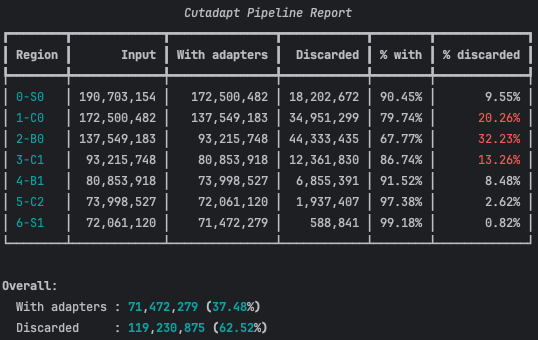
\includegraphics[width=\textwidth]{figures/qc-poor-selection-report.png}
\caption{Example report for a poor selection with only 37\% read retention. The report highlights the problematic region where more than 10\% of the reads are lost during codon assignment, which typically indicates a barcode-definition mismatch, low read quality reads, or an unexpected sequence architecture.}
\label{fig:figure4}
\end{figure}

\begin{figure}[H]
\centering
%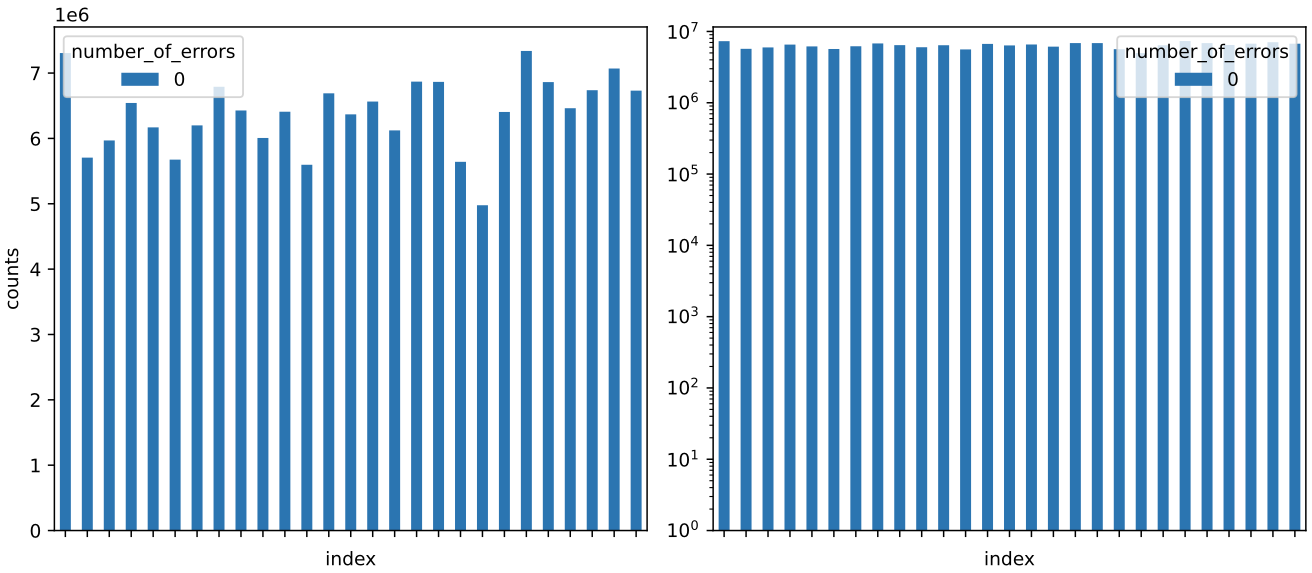
\includegraphics[width=\textwidth]{figures/qc-stacked-barplots.png}
%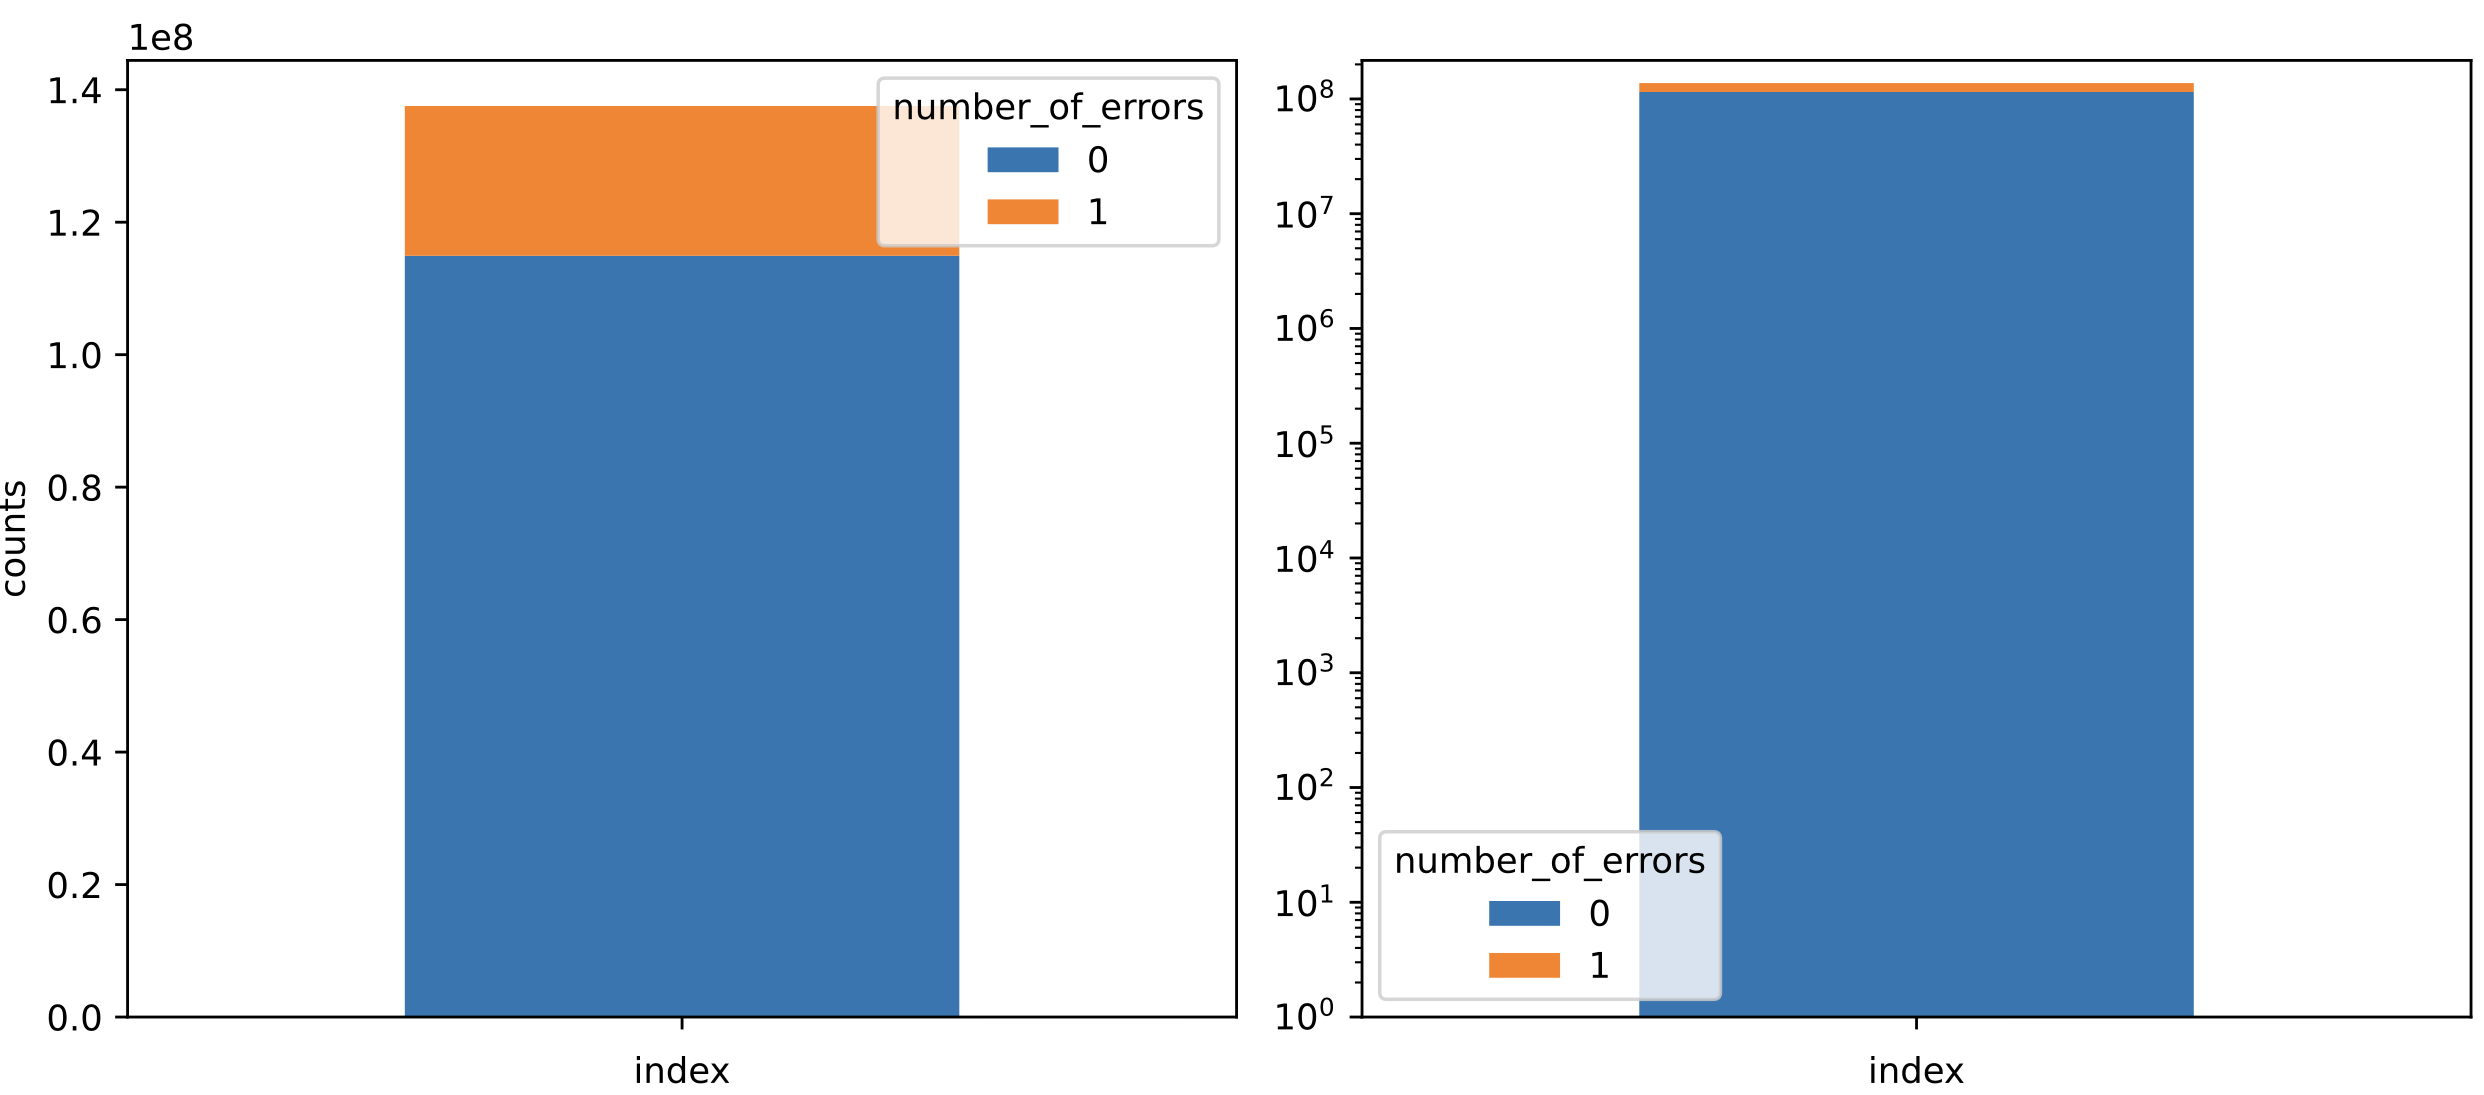
\includegraphics[width=\textwidth]{figures/qc-stacked-barplots-with-errors.png}
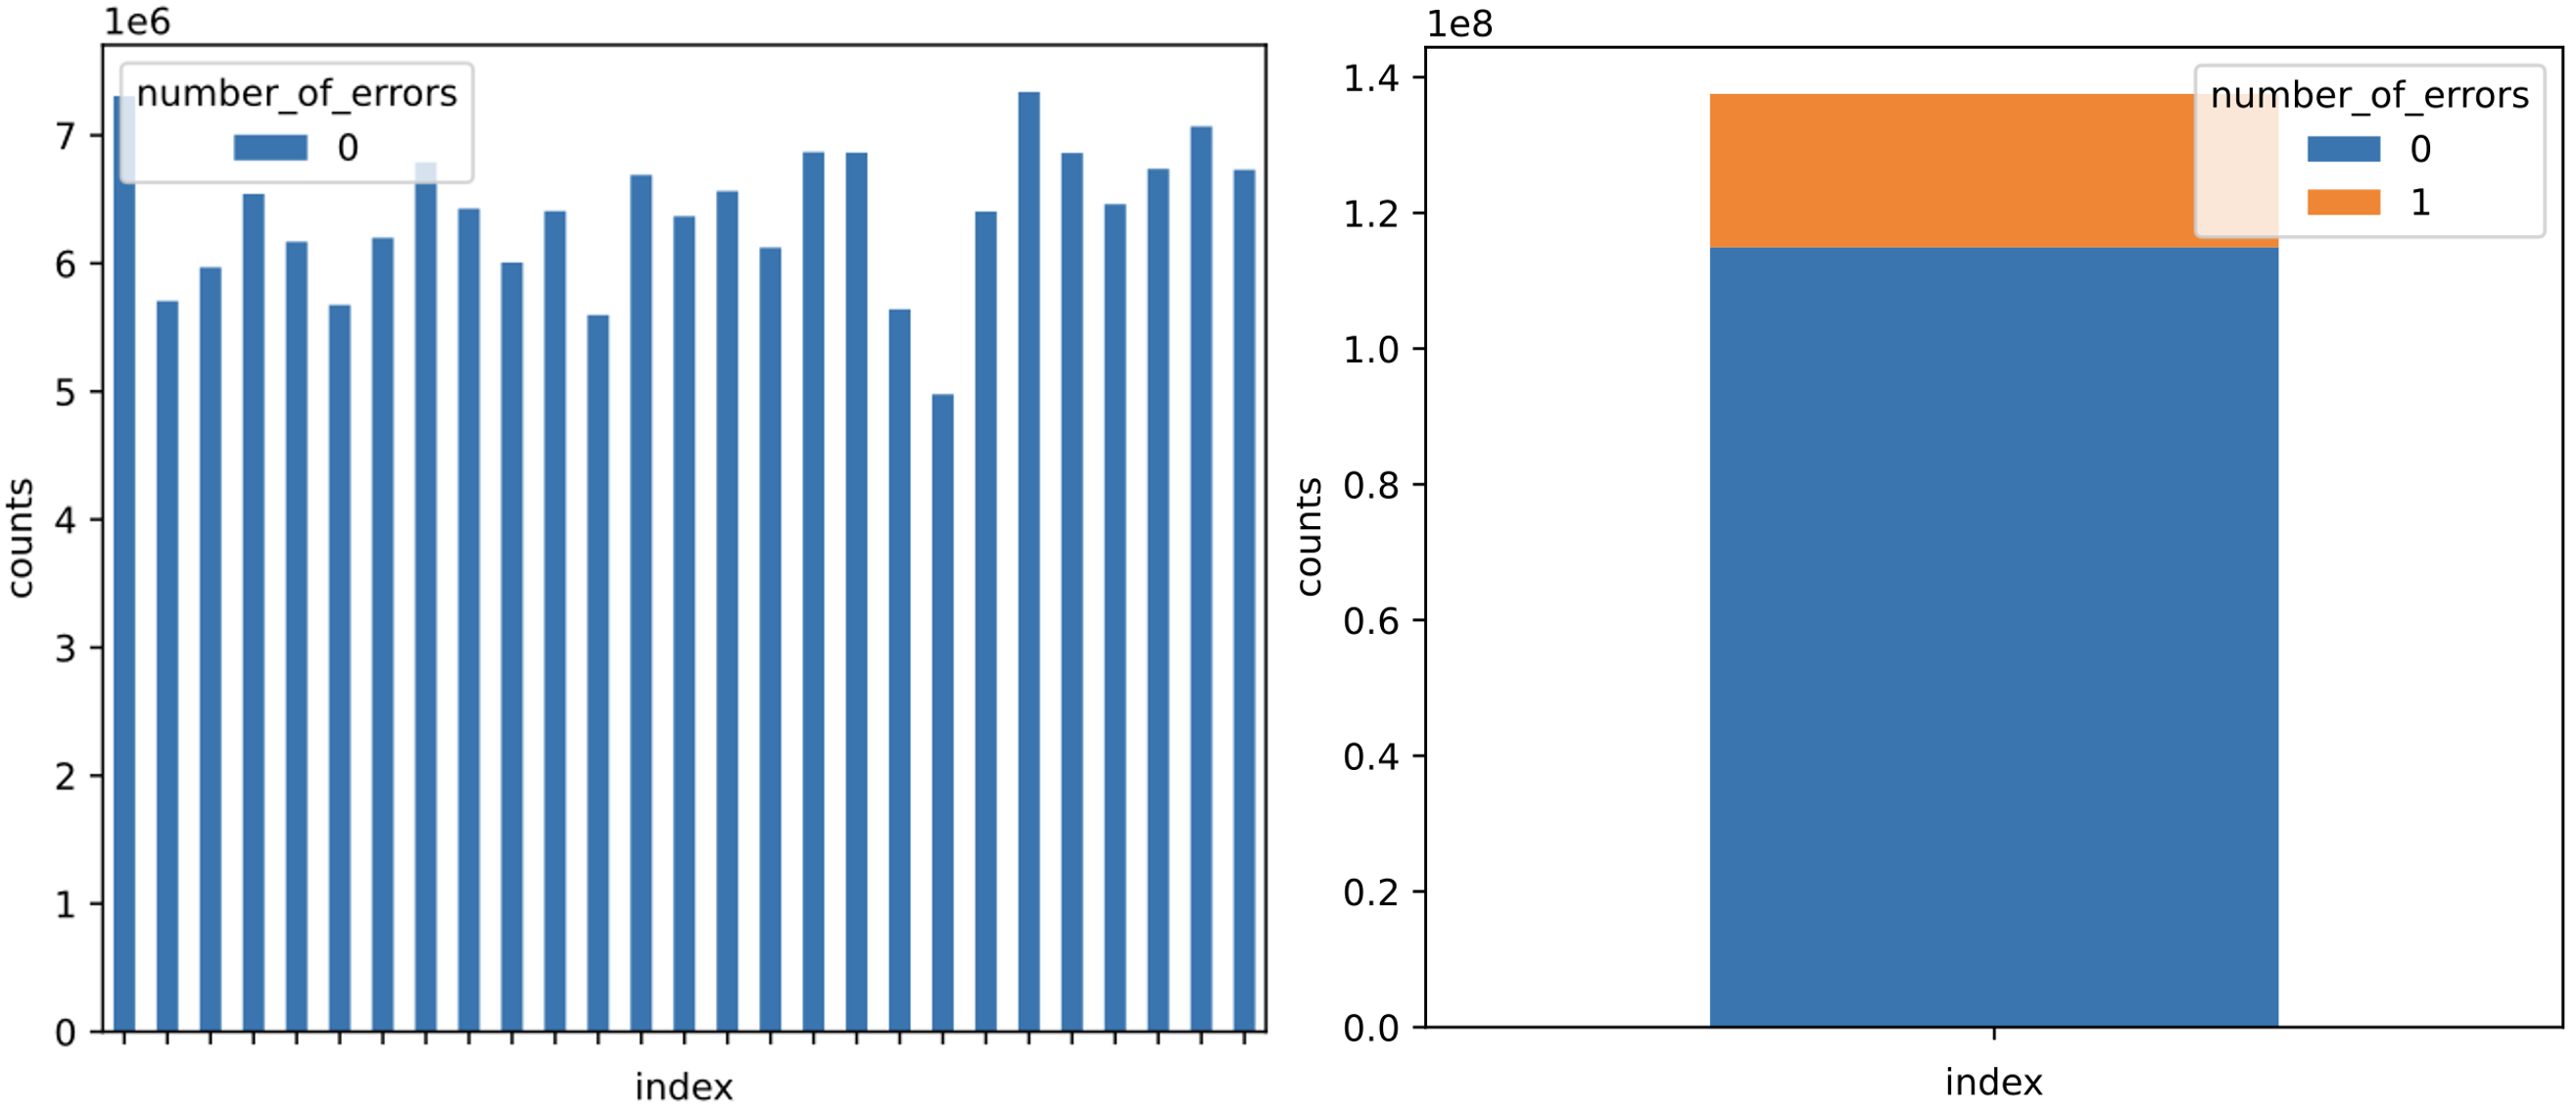
\includegraphics[width=\textwidth]{figures/qc-stacked-barplot-composite.png}
\caption{Quality-control plots showing log-transformed read counts for barcode and constant-region sequences after demultiplexing. The left panel displays the number of reads mapped to building block 0 (BB0) barcode indices, while the right panel shows the number of reads mapped to the constant region 0 index. For the barcode region, exact matching was required, and therefore all mapped reads have 0 sequencing errors. For the constant region, up to one sequencing error was permitted during matching. Reads matching exactly are shown in blue, whereas reads matching with one sequencing error are shown in orange. Strong dropout of individual barcode indices or an increased proportion of one-error matches may indicate issues with oligonucleotide synthesis, sequencing quality, or library preparation.}
\label{fig:figure5}
\end{figure}

\newpage

\protocolstep{13}{Process demultiplexing results into count tables}

Once the quality-control inspection is satisfactory, aggregate the demultiplexed reads into selection-level count tables: 

\begin{lstlisting}
# Process demultiplexing output and generate count tables
delt-hit demultiplex process --config_path=$CONFIG_PATH

# Also export flattened per-selection count files
delt-hit demultiplex process --config_path=$CONFIG_PATH --as_files=True

delt-hit demultiplex process --config_path=$CONFIG_PATH --as_files=True --sort_by_counts=False
\end{lstlisting}

<PAUSE POINT> The generated count tables for each selection are saved in a standardized format for visualization and enrichment analysis.

\subsection{Phase 3 | Data visualization and interpretation}

\textbf{TIMING:} 10--30 min

<CRITICAL>: This phase demonstrates how demultiplexing results can be visualised in the interactive dashboard. 

\protocolstep{14}{Launch the interactive analysis dashboard}
Launch the interactive dashboard and explore count distributions. Open the local server in a web browser, typically at \url{http://localhost:8050} (see print statement in the terminal). Stop the server with \texttt{Ctrl+C} or by closing the terminal. An example dashboard view is shown in Figure~\ref{fig:figure7}.


\begin{lstlisting}
delt-hit dashboard --config_path=$CONFIG_PATH \
  --counts_path=<name>/selections/<selection_name>/counts.txt

# Dash is running on http://127.0.0.1:8050/  # copy paste into browser
# * Serving Flask app 'delt_hit.cli.dashboard.api'
# * Debug mode: on
\end{lstlisting}


<CRITICAL> The command accepts counts provided as a \texttt{.txt} file, so custom normalized count tables can also be visualized by passing \texttt{--counts\_path} and, if needed, \texttt{--selection\_name}. Use the default folder hierarchy produced by \texttt{delt-hit demultiplex process}. If a custom \texttt{counts.txt} file is provided, also pass the selection name exactly as specified in the selection sheet.

\begin{figure}[htbp]
\centering
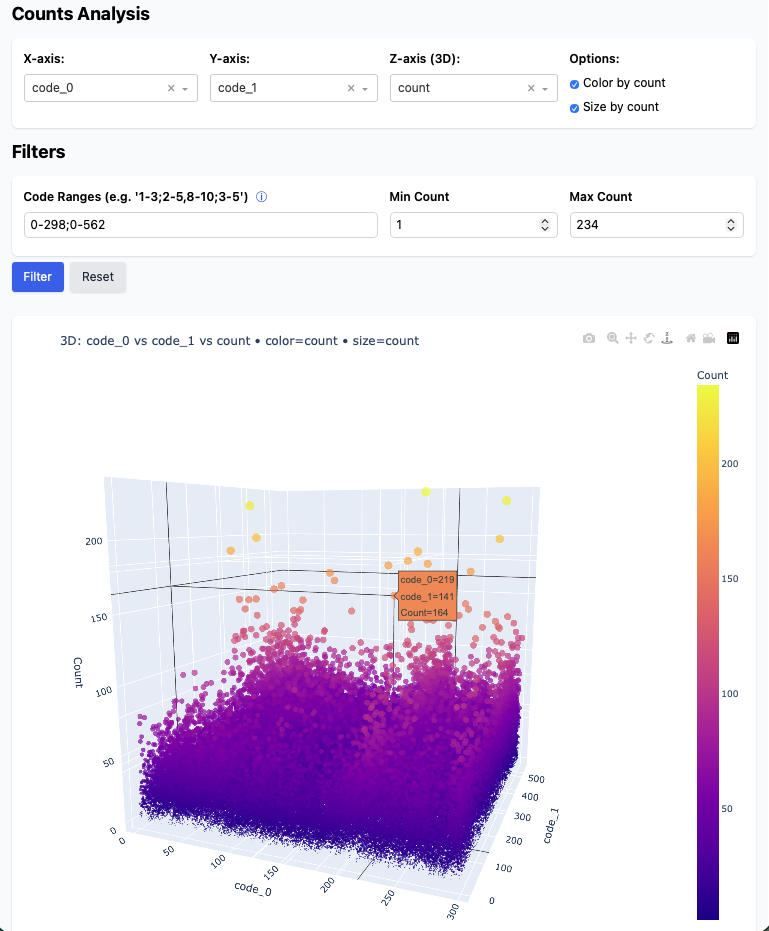
\includegraphics[width=\textwidth]{figures/dashboard.png}
\caption{Interactive dashboard interface for exploring raw count data and experimental metadata. The dashboard provides count-distribution views, filtering controls, and selection-level context to support rapid inspection of demultiplexing outputs before downstream statistical analysis.}
\label{fig:figure7}
\end{figure}

\newpage

\subsection{Phase 4 | Selection enumeration and enrichment analysis}

\textbf{TIMING:} \textless{}1 min
 
<CRITICAL>: This phase generates chemical structures and molecular properties for the top enriched compounds in a selected experiment. 2D representations of the reaction schemes, building blocks and enriched compounds as well as molecular property plots as shown in Figure~\ref{fig:figure2} and Figure~\ref{fig:figure3} can provide visual support for the analysis of selection results. 


\protocolstep{15}{Enumerate top compounds from a selection}
Generate chemical structures for the top enriched compounds in a selected experiment. Visualize the reaction graph to verify the chemical structure of library components.

\begin{lstlisting}
delt-hit visualize enumerate --config_path=$CONFIG_PATH
\end{lstlisting}

Enumerate the \texttt{top\_n} compounds by count for the selected experiment. 

\begin{lstlisting}
delt-hit library enumerate \
  --config_path=$CONFIG_PATH \
  --counts_path=<name>/selections/<selection_name>/counts.txt \
  --top_n=<top_n> \
  --library_name=<library_name>
\end{lstlisting}


\begin{figure}[htbp]
\centering
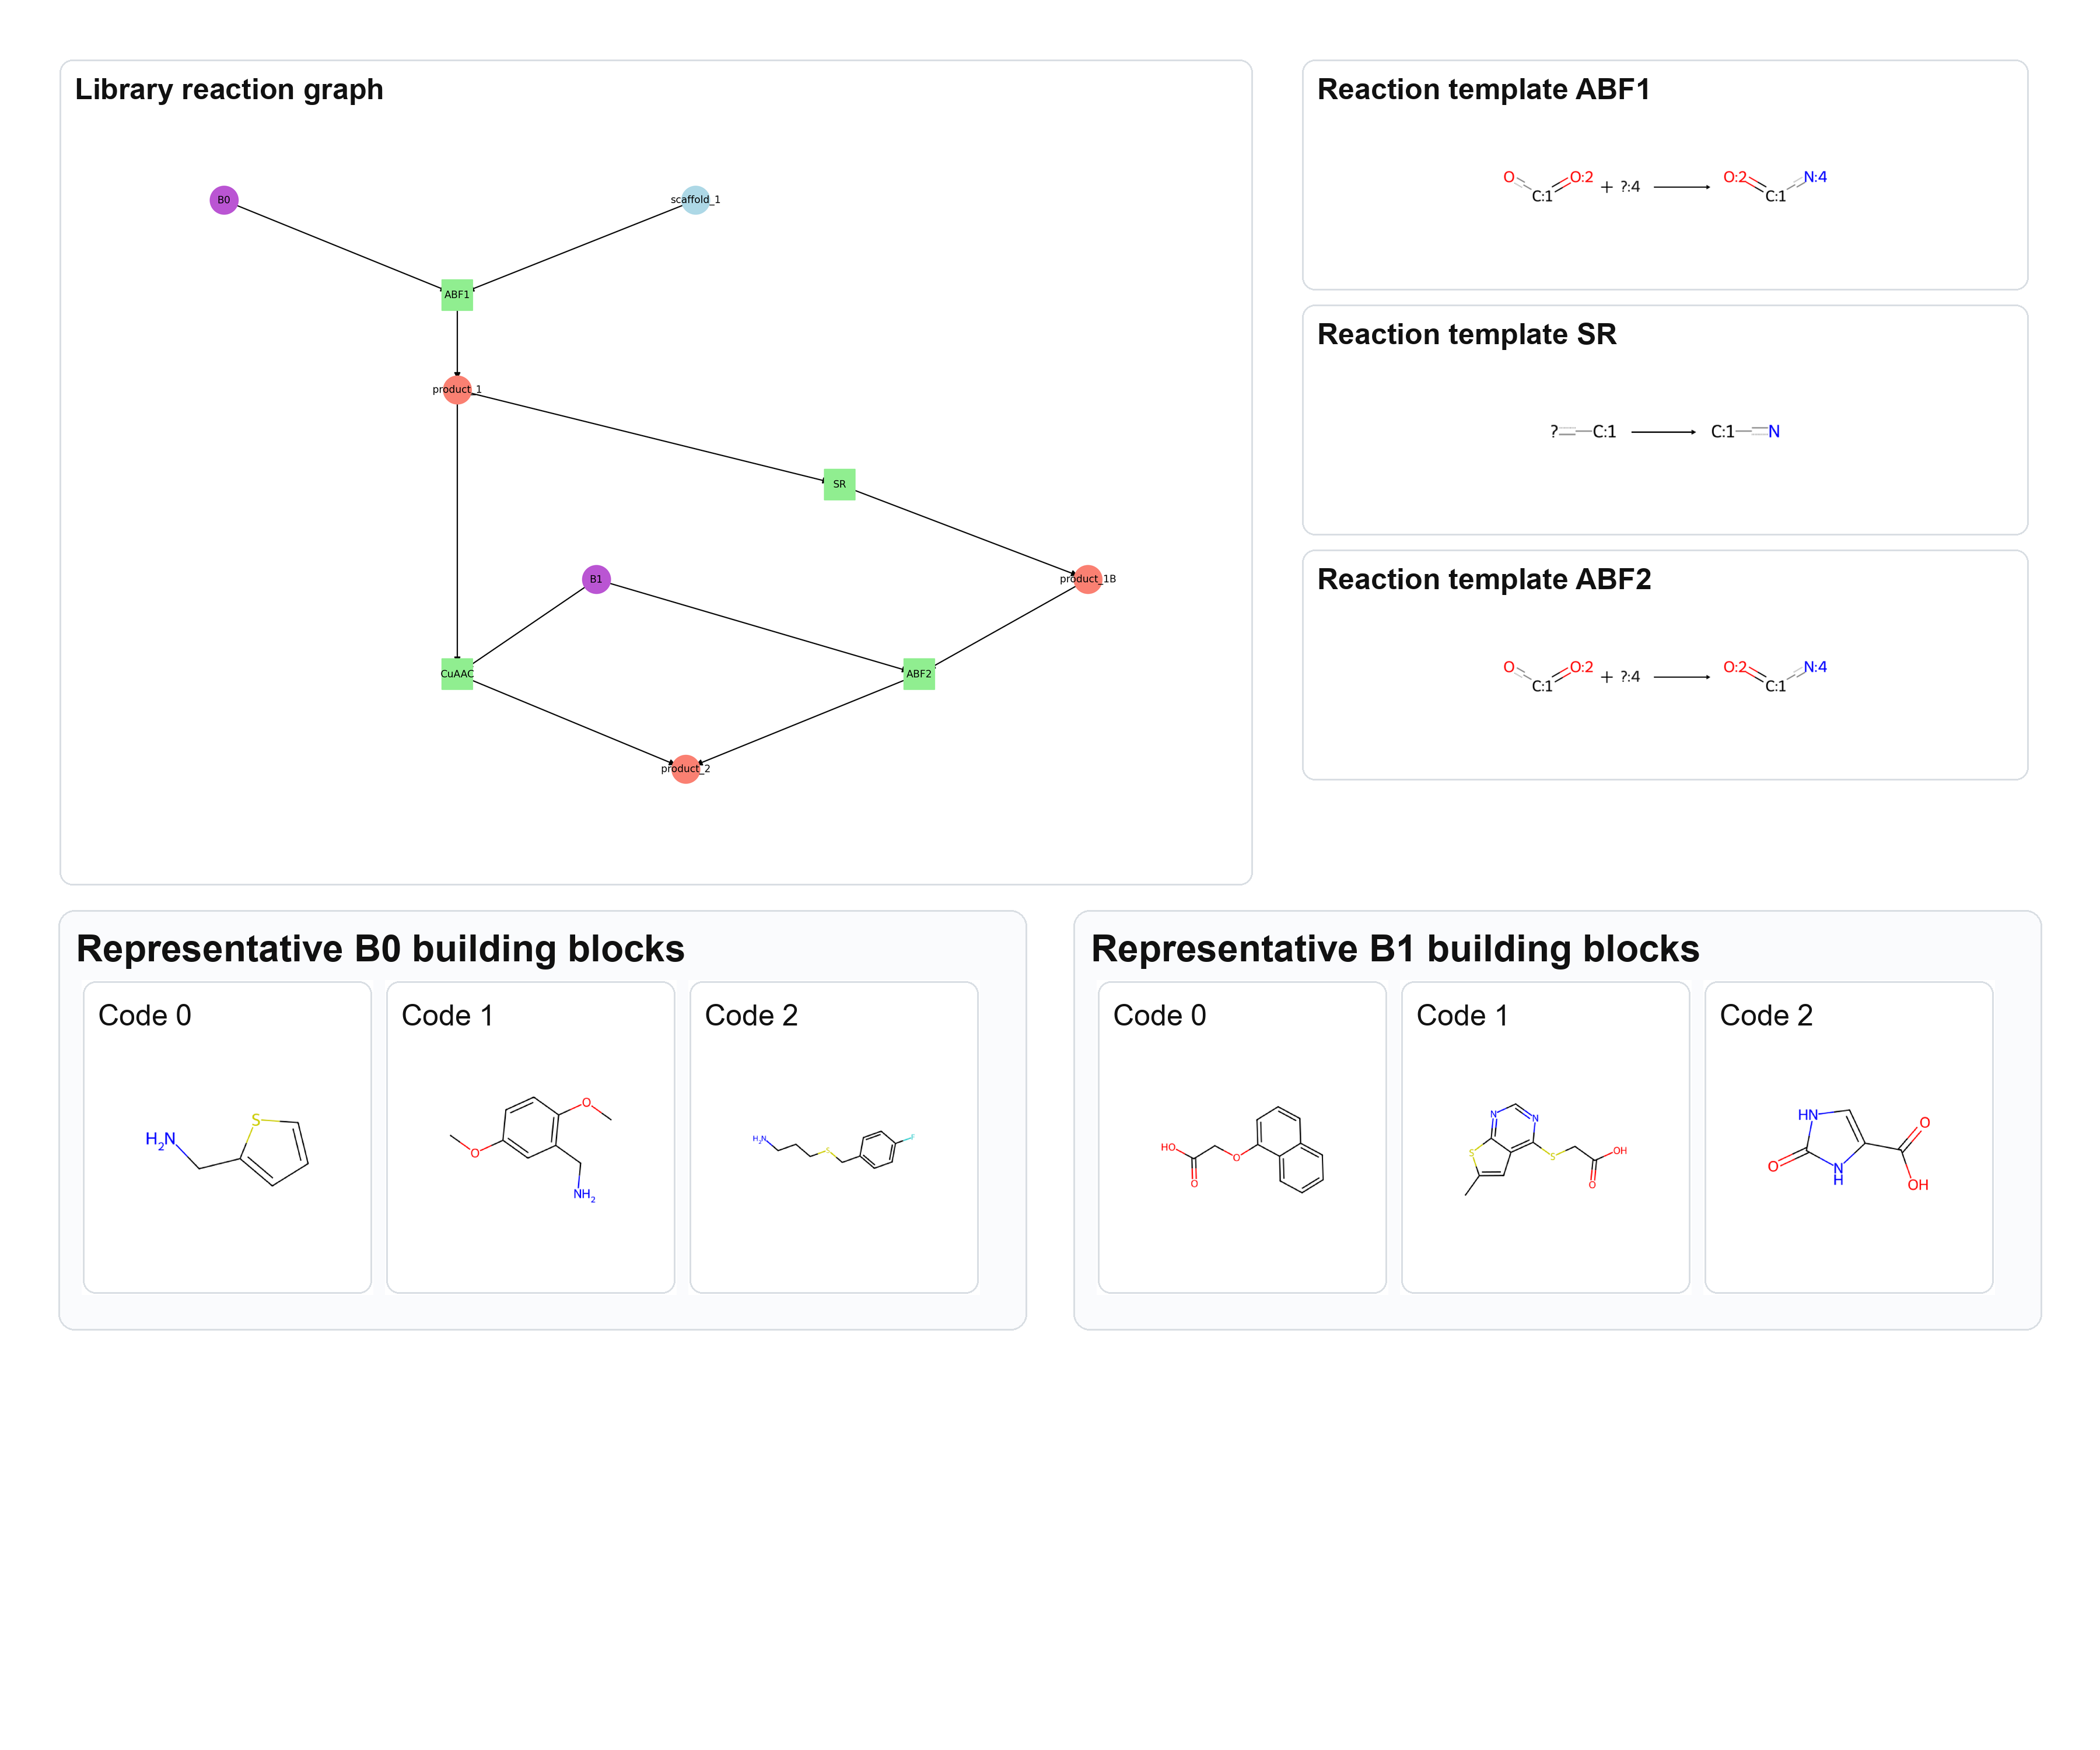
\includegraphics[width=\textwidth]{figures/enumeration-summary.png}
\caption{Composite summary of the enumeration visualization command outputs from the single-display example workflow. The main panel shows the library reaction graph, alongside representative reaction templates and example \texttt{B0} and \texttt{B1} building blocks generated during selection-focused library enumeration.}
\label{fig:figure2}
\end{figure}

<CRITICAL>: Library enumeration requires advanced knowledge of SMIRKS, and library-specific adjustments are often necessary.

\textbf{$\blacklozenge$ Troubleshooting}

\newpage

\protocolstep{16}{Visualize and calculate molecular properties of top hits}

Visualize the chemical structure of the most observed compounds:

\begin{lstlisting}
delt-hit visualize library --config_path=$CONFIG_PATH --library_name=<library_name>
\end{lstlisting}

Calculate molecular descriptors for chemical-space characterization:

\begin{lstlisting}
delt-hit library properties --config_path=$CONFIG_PATH --library_name=<library_name>
\end{lstlisting}


\begin{figure}[H]
\centering
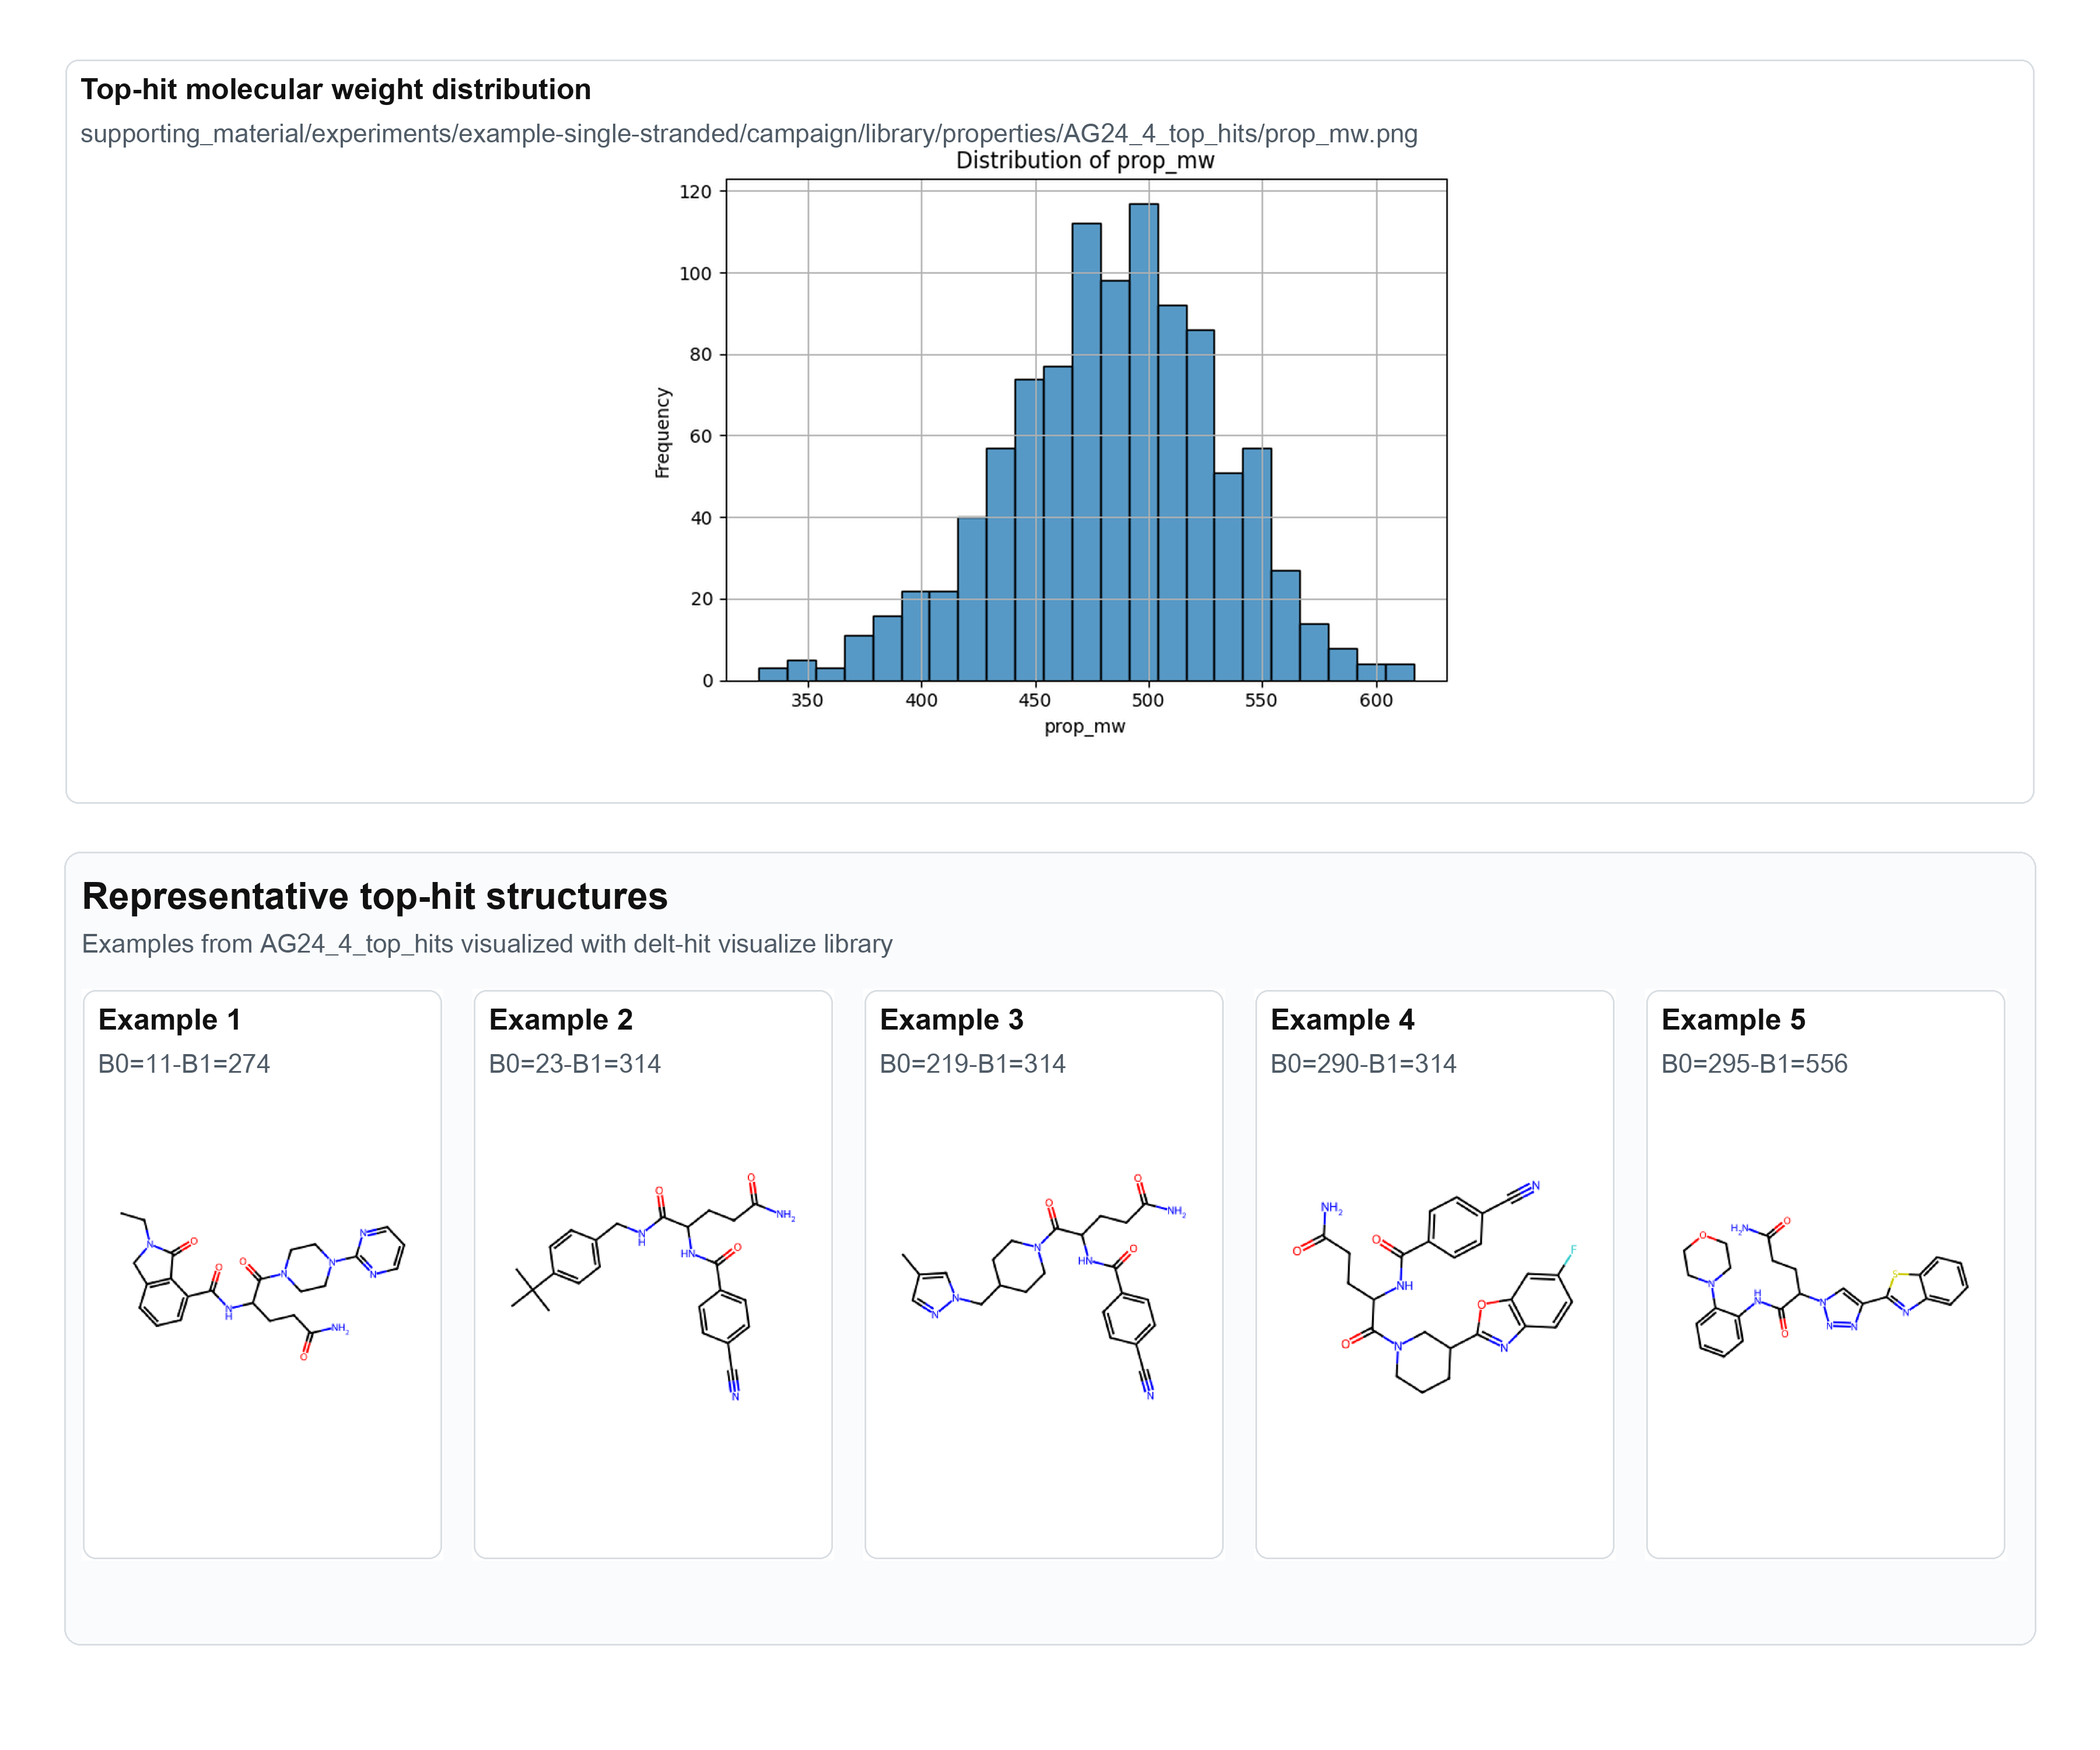
\includegraphics[width=\textwidth]{figures/top-hit-properties-and-structures.png}
\caption{Molecular property and structure summary for the enumerated \texttt{AG24\_4\_top\_hits} collection. The left panel shows the molecular-weight distribution from the example output, and the right panels show four representative structure renderings produced by \texttt{delt-hit visualize library}.}
\label{fig:figure3}
\end{figure}


\subsection{Phase 5 | Statistical analysis and hit identification}

\textbf{TIMING:} \textless{}5 min

<CRITICAL>: This phase identifies enriched library members by comparing selection conditions using established statistical methods.

\protocolstep{17}{Define statistical comparisons}

Using the information from the selection sheet, create a dedicated YAML configuration file that specifies which selections to compare. Comparisons across different selection runs and runs derived from multiple sequencing files are supported. Following the template below, organize the file as a list of \texttt{experiments}, where each experiment defines one named comparison and contains a \texttt{selections} list. Each selection entry specifies the selection name, the corresponding \texttt{counts\_path}, and a \texttt{group} label indicating whether that selection belongs to the control or condition set for the comparison. An example for the single-display workflow (see Box~2) is given below for orientation. 


\begin{lstlisting}
# analysis.yaml -- general structure
experiments:
- name: <experiment_name>        # referenced as --name in commands
  selections:
    - name: <selection_name>
      counts_path: <name>/selections/<selection_name>/counts.txt
      group: control             # or "condition"
    - ...
\end{lstlisting}

Example for the single-display workflow (see Box~2):

\begin{lstlisting}
# analysis.yaml
experiments:
- name: condition_vs_control
  selections:
    - name: AG24_4
      counts_path: campaign/selections/AG24_4/counts.txt
      group: control
    - name: AG24_5
      counts_path: campaign/selections/AG24_5/counts.txt
      group: control
    - name: AG24_6
      counts_path: campaign/selections/AG24_6/counts.txt
      group: control
    - name: AG24_13
      counts_path: campaign/selections/AG24_13/counts.txt
      group: condition
    - name: AG24_14
      counts_path: campaign/selections/AG24_14/counts.txt
      group: condition
    - name: AG24_15
      counts_path: campaign/selections/AG24_15/counts.txt
      group: condition
\end{lstlisting}

\protocolstep{18}{Perform enrichment analysis with statistical methods}
<CRITICAL>: DELT-Hit supports three statistical approaches for identifying enriched compounds. Methods A, B, and C each generate an R script that can be executed directly or adapted further. Use method C for experiments without replicates and any of the three methods for evaluation settings where replicates are available. The generated files report the enrichment score for each compound and, where applicable, method-specific parameters such as log fold change or \textit{P} values.

A. Simple counts method

<CRITICAL>: This method averages counts across replicates within each group and computes a direct enrichment score from the difference between the condition and control groups. While it does not provide formal significance testing, it is useful for comparisons involving replicates as a straightforward ranking approach.

(i) Generate the R script for the counts-based analysis:
\begin{lstlisting}
delt-hit analyse enrichment --analysis_config=<analysis_config> \
  --save_dir=<save_dir> --name=<experiment_name> --method=counts
\end{lstlisting}

(ii) Execute the generated R script:
\begin{lstlisting}
Rscript --vanilla <save_dir>/counts/<experiment_name>/enrichment_counts.R
\end{lstlisting}


B. edgeR method

<CRITICAL>: This method applies RNA-seq-derived statistical modeling with empirical Bayes shrinkage, reports false-discovery-rate-corrected \textit{P} values, and provides normalized count tables for each selection. Use it alongside enrichment ranking as a significance-annotation layer, when replicates are available. An exemplary output for this method is given in Table~\ref{tab:table12}.

(i) Generate the R script for edgeR statistical analysis:
\begin{lstlisting}
delt-hit analyse enrichment --analysis_config=<analysis_config> \
  --save_dir=<save_dir> --name=<experiment_name> --method=edgeR
\end{lstlisting}

(ii) Execute the generated R script:
\begin{lstlisting}
Rscript --vanilla <save_dir>/edgeR/<experiment_name>/enrichment_edgeR.R
\end{lstlisting}


C. Normalized z-score method

<CRITICAL>: This method computes the per-compound score for an individual selection following Faver et al.\cite{faver_quantitativecomparisonenrichment_2019} and can be used for experiments without replicates. The generated output contains both the raw \texttt{z\_score} and the depth-normalized \texttt{norm\_z\_score}, defined as $z\_score / \sqrt{n}$ and used for ranking. 

(i) Generate the R script for normalized z-score analysis:
\begin{lstlisting}
delt-hit analyse enrichment --config_path=$CONFIG_PATH \
  --counts=<name>/selections/<selection_name>/counts.txt \
  --save_dir=<save_dir> --name=<selection_name> --method=z_score
\end{lstlisting}

(ii) Execute the generated R script:
\begin{lstlisting}
Rscript --vanilla <save_dir>/z_score/<selection_name>/enrichment_z_score.R
\end{lstlisting}


\textbf{$\blacklozenge$ Troubleshooting}


<CRITICAL> Guidelines for result interpretation are given below. Always examine replicate correlation plots to verify data quality before interpreting hit lists. Poor correlation may indicate technical problems or batch effects. 

\begin{itemize}
  \item Higher enrichment scores indicate stronger enrichment
  \item Some methods additionally report a log fold change relative to a control; LogFC \textgreater{} 0 corresponds to enrichment relative to the control
  \item FDR \textless{} 0.05 indicates statistically significant enrichment for methods that report adjusted \textit{P} values
  \item High replicate correlation ($R^2 > 0.7$) indicates good experimental consistency
\end{itemize}


\begin{table}[htbp]
\centering
\caption{Hit identification by edgeR. Shown compounds are for FDR\textless{}0.05 and sorted by logFC to identify the top hits.}
\label{tab:table12}
\begin{tabular}{lllllll}
\toprule
code\_1 & code\_2 & logFC & logCPM & LR & PValue & FDR \\
\midrule
94 & 472 & 9.76658103 & 4.65399379 & 140.973181 & 1.63E-32 & 2.99E-29 \\
94 & 337 & 9.52452422 & 4.41931582 & 128.115071 & 1.06E-29 & 9.38E-27 \\
250 & 250 & 9.50138143 & 4.39920396 & 136.048263 & 1.95E-31 & 2.62E-28 \\
250 & 523 & 9.46551754 & 4.36448577 & 134.035088 & 5.37E-31 & 6.34E-28 \\
94 & 364 & 9.29500646 & 4.19806216 & 117.172728 & 2.63E-27 & 1.35E-24 \\
250 & 208 & 9.2845154 & 5.99659857 & 173.194896 & 1.48E-39 & 2.05E-35 \\
250 & 337 & 9.06687397 & 3.98375428 & 115.539372 & 6.00E-27 & 2.80E-24 \\
94 & 341 & 8.99590166 & 3.91723403 & 113.847311 & 1.41E-26 & 6.00E-24 \\
250 & 414 & 8.99240694 & 3.90981012 & 105.694583 & 8.60E-25 & 2.69E-22 \\
250 & 96 & 8.92430743 & 8.02773969 & 203.793994 & 3.10E-46 & 2.36E-41 \\
\bottomrule
\end{tabular}
\end{table}



\subsection{Phase 6 | Full library enumeration and machine learning representations}

\textbf{TIMING:} 15 min--2 h

<CRITICAL>: This phase performs full-library enumeration and generates molecular representations for downstream machine-learning applications. These steps are optional. When only a focused subset is needed, the filtered-enumeration route in Step~15 usually provides a faster alternative to full-library processing.

\protocolstep{19}{Enumerate the full library}

Generate molecular representations of all library members: 

\begin{lstlisting}
delt-hit library enumerate --config_path=$CONFIG_PATH
\end{lstlisting}

\protocolstep{20}{Calculate molecular properties for the full library}

Compute molecular properties for all enumerated compounds:

\begin{lstlisting}
delt-hit library properties --config_path=$CONFIG_PATH
\end{lstlisting}

\protocolstep{21}{Generate molecular representations for machine learning}

Create standardized chemical representations compatible with common machine-learning frameworks. Two methods tailored for different applications are available. Method A (\texttt{morgan}) generates Morgan circular fingerprints (2048-bit vectors), which are useful for similarity analysis. Method B (\texttt{bert}) generates transformer-based molecular embeddings (768-dimensional vectors) for deep-learning applications.


A. Morgan fingerprints

(i) Generate Morgan fingerprints (Approx. 600-1000 compounds/s):
\begin{lstlisting}
delt-hit library represent --method=morgan --config_path=$CONFIG_PATH
\end{lstlisting}

B. BERT embeddings

(i) Generate BERT embeddings (Approx. 600-1000 compounds/s):
\begin{lstlisting}
delt-hit library represent --method=bert --config_path=$CONFIG_PATH
\end{lstlisting}
